
%%%%%%%%% PROPOSAL -- 15 pages (including Prior NSF Support)

\section{Introduction}
In the last decade, our knowledge of the neutrino has grown exponentially. Low-energy neutrino ($\lesssim$10~MeV) experiments have been instrumental in proving that neutrinos oscillate and therefore have mass. Although our picture of the physics is much clearer now, many questions remain. One of the most tantalizing is the question of the Majorana nature of the neutrino, or, stated differently, whether the neutrino is its own antiparticle. If the neutrino is Majorana then, in models of leptogenesis, the neutrino is responsible for the matter-antimatter  asymmetry we observe in the universe today. This is why both the Multidivisional Neutrino Study from 2004\cite{numatrix}  and this year's National Academy report on nuclear physics\cite{national2012Nuclear} highlight this as a key question to be addressed in the next generation of neutrino experiments.

The only feasible experimental probes of the Majorana nature of the neutrino are low-energy neutrino experiments searching for the rare nuclear process neutrinoless double-beta decay (\zeronu). The next generation of these experiments has started to take data, with first results from EXO\cite{EXO2012} and KamLAND-Zen\cite{KZ2nu} presented in the last year. These experiments are designed either to confirm or refute the claimed observation in \isoge\cite{KKK2006}. The first experiment designed to have the sensitivity to push beyond these bounds into the uncharted territory of the inverted neutrino mass hierarchy is the CUORE experiment. 

CUORE is a two-staged experiment, which builds on the experience of the successful CUORICINO experiment\cite{CC2008}. It uses TeO$_{2}$ crystals instrumented as bolometers to search for \zeronu~in \isomain. The first stage of the experiment, CUORE-0, started in the fall of 2012 with the commencement of data taking from the first tower of CUORE crystals. This makes it an excellent time for a young PI to join the experiment, gain experience in this unique detector technology, and make a valuable contribution to both the hardware and the analysis.

The PI of this proposal has considerable experience in low-energy neutrino physics from their work on the KamLAND and Double Chooz experiments. In particular, the PI is very familiar with the modeling of backgrounds from natural radioactivity, in addition to having extensive experience simulating backgrounds produced in muon spallation. The final sensitivity of the \zeronu~analysis depends almost entirely on the understanding of the backgrounds; therefore, this knowledge transfers very effectively to the CUORE analysis.

There are two tasks on CUORE that need more resources as CUORE makes the transition from construction to commissioning and data taking. These are the slow monitoring system and the Monte Carlo (MC). Because CUORE represents a leap forward in size for this technology, the tools developed for CUORICINO for both of these systems are insufficient. The PI performed performed these same job on Double Chooz, so brings experience from commissioning, operating, and analyzing data from that detector, and is well positioned to lead these efforts.    

The hardware and analysis tasks outlined in this proposal fit in nicely with the PI's skills and the project's needs. The group, the PI with  postdoc Dr. Kevin Hickerson, graduate student Erin Hansen and undergraduate Elizabeth Friedman are ready to start the proposed tasks. Furthermore, these tasks complement the work being done at UCLA  by Professor Huan Huang's group on the front-end electronics, and this award would create a quorum for analysis at UCLA. The timescale of the proposed work fits well with the overall schedule of the experiment. In the first year of the grant, the slow monitoring interfaces would be written and the data from CUORE-0 analyzed. In year two of the grant, the full CUORE detector is commissioned, and this is followed by the first results from CUORE in year three of the grant. This schedule, the details of the physics, and the proposed work are outlined further in the body of this proposal.


\section{Motivation}
\subsection{Neutrino Oscillation: Neutrino Mass to Precision Measurements}
The standard model neutrino is a massless particle which comes in three weak flavor eigenstates: electron, muon, and tau. It was realized early on that if the mass eigenstates of the neutrino do not correspond to the interaction states then a classic quantum oscillation scenario develops. Pontecorvo first proposed a neutrino oscillation scenario of  $\nu-\bar{\nu}$, which was similar to the oscillation seen in the quarks with systems like $K^{0}-\bar{K^{0}}$ \cite{Pontecorvo:1957qd}. The flavor oscillations that we now observe correspond to the scenario first outlined by Maki, Nakagawa, and Sakata (MNS)\cite{Maki:1962mu}. 

In the MNS scenario, the flavor eigenstates of the weak interaction are described by the superposition of the mass eigenstates as
\begin{equation}
\left| \nu_{\alpha} \right> = \sum_{j} U^*_{\alpha j} \left| \nu_{j}\right>,
\end{equation}
where the matrix describes the mixing of the mass eigenstates. This matrix U is called the MNSP matrix in honor of the original formulators. It is parameterized by three mixing angles and at least one complex phase, $\delta$:
\begin{equation}
\label{eq:osc_matrix}
\begin{array}{l c l}
U_{\alpha j} & = &
\begin{pmatrix}
1 & 0 & 0 \\
0 & \cos \theta_{23} & \sin \theta_{23}\\ 
0 & -\sin \theta_{23} & \cos \theta_{23} 
\end{pmatrix}
\begin{pmatrix}
\cos \theta_{13} & 0 &  \sin \theta_{13}e^{-i\delta}\\
0 & 1 & 0\\ 
-\sin \theta_{13}e^{i\delta} & 0 & \cos \theta_{13}
\end{pmatrix}
\begin{pmatrix} 
\cos \theta_{12} & \sin \theta_{12}  & 0\\ 
-\sin \theta_{12} & \cos \theta_{12}  & 0\\
0 & 0 & 1
\end{pmatrix} 
\\
\\
 & \times & \begin{pmatrix}
 e^{i\xi_{1}/2} & 0 & 0\\ 
0 & e^{i\xi_{2}/2} & 0\\ 
0 & 0 & 1
\end{pmatrix}
\end{array}.
\end{equation}
The additional complex phases,  $\xi_1$ and $\xi_2$, are only relevant for Majorana neutrinos. 

The discovery of neutrino oscillation and now the precision measurement of the mixing angles with the corresponding mass differences are the two great accomplishments of neutrino oscillation experiments. With the measurement of $\theta_{13}$, all angles in the MNSP matrix are now known. Therefore, the phases are now the main focus of the neutrino community. The only phase that can be measured in an oscillation experiment is $\delta$. The PI has contributed to one proposed experiment, DAE$\delta$ALUS\cite{Alonso:2010fs}, which aims to create a pion decay-at-rest beam using cyclotron technology. The PI has also been involved in the precursor experiment to DAE$\delta$ALUS, IsoDAR, which proposes to uses a smaller cyclotron to make a $^{8}$Li isotope decay-at-rest antineutrino beam to search for sterile neutrinos. This is one future experiment that the group is working on mainly through small undergraduate projects. The PI would like to continue working on these future endeavors; however, the focus of this proposal is the Majorana phases whose combined effect can be observed in \zeronu~experiments. These experiments analyze signals and backgrounds in the 0.5-5~MeV region and it is in this energy range where the PI has the greatest expertise.

\subsection{Neutrinoless Double Beta Decay}

\begin{figure}
\begin{center}
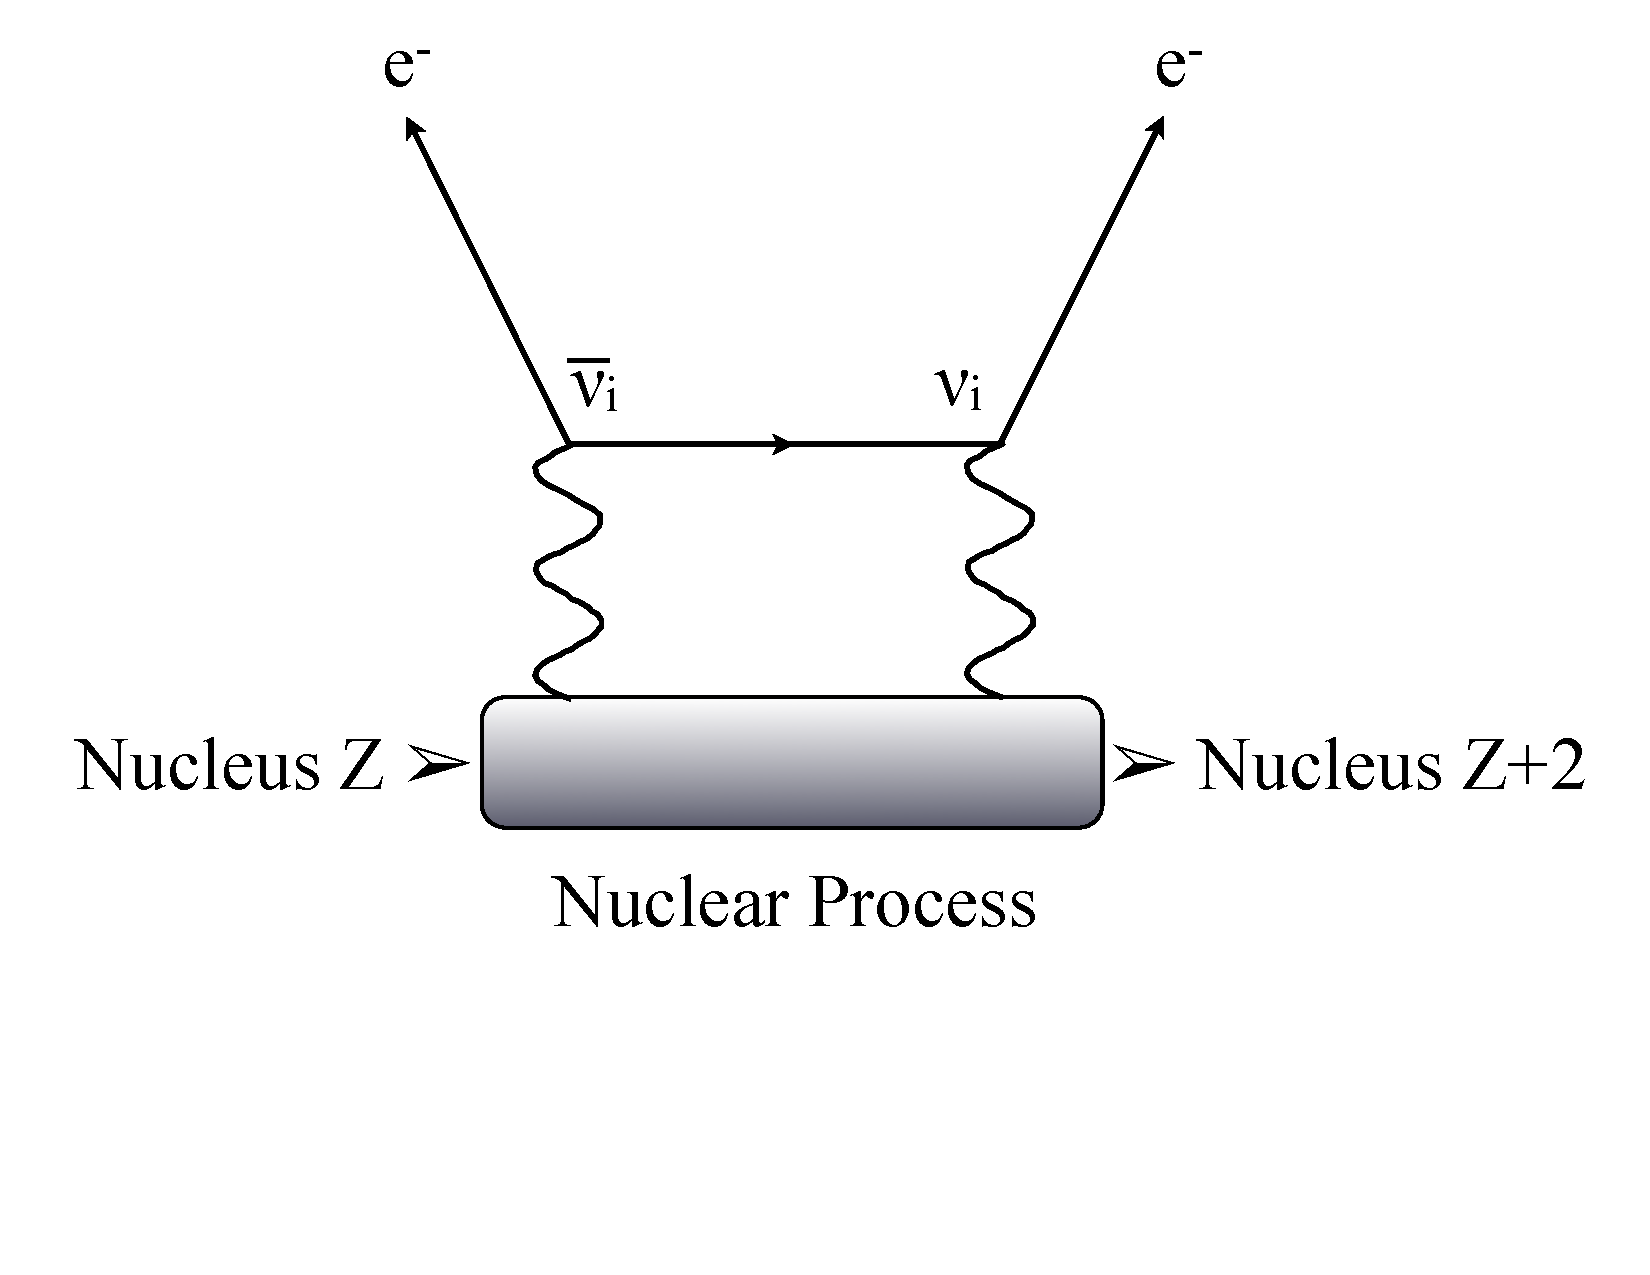
\includegraphics[trim = 0mm 10mm 0mm 5mm, clip, width=0.3\columnwidth]{figs/0nBB.pdf} 
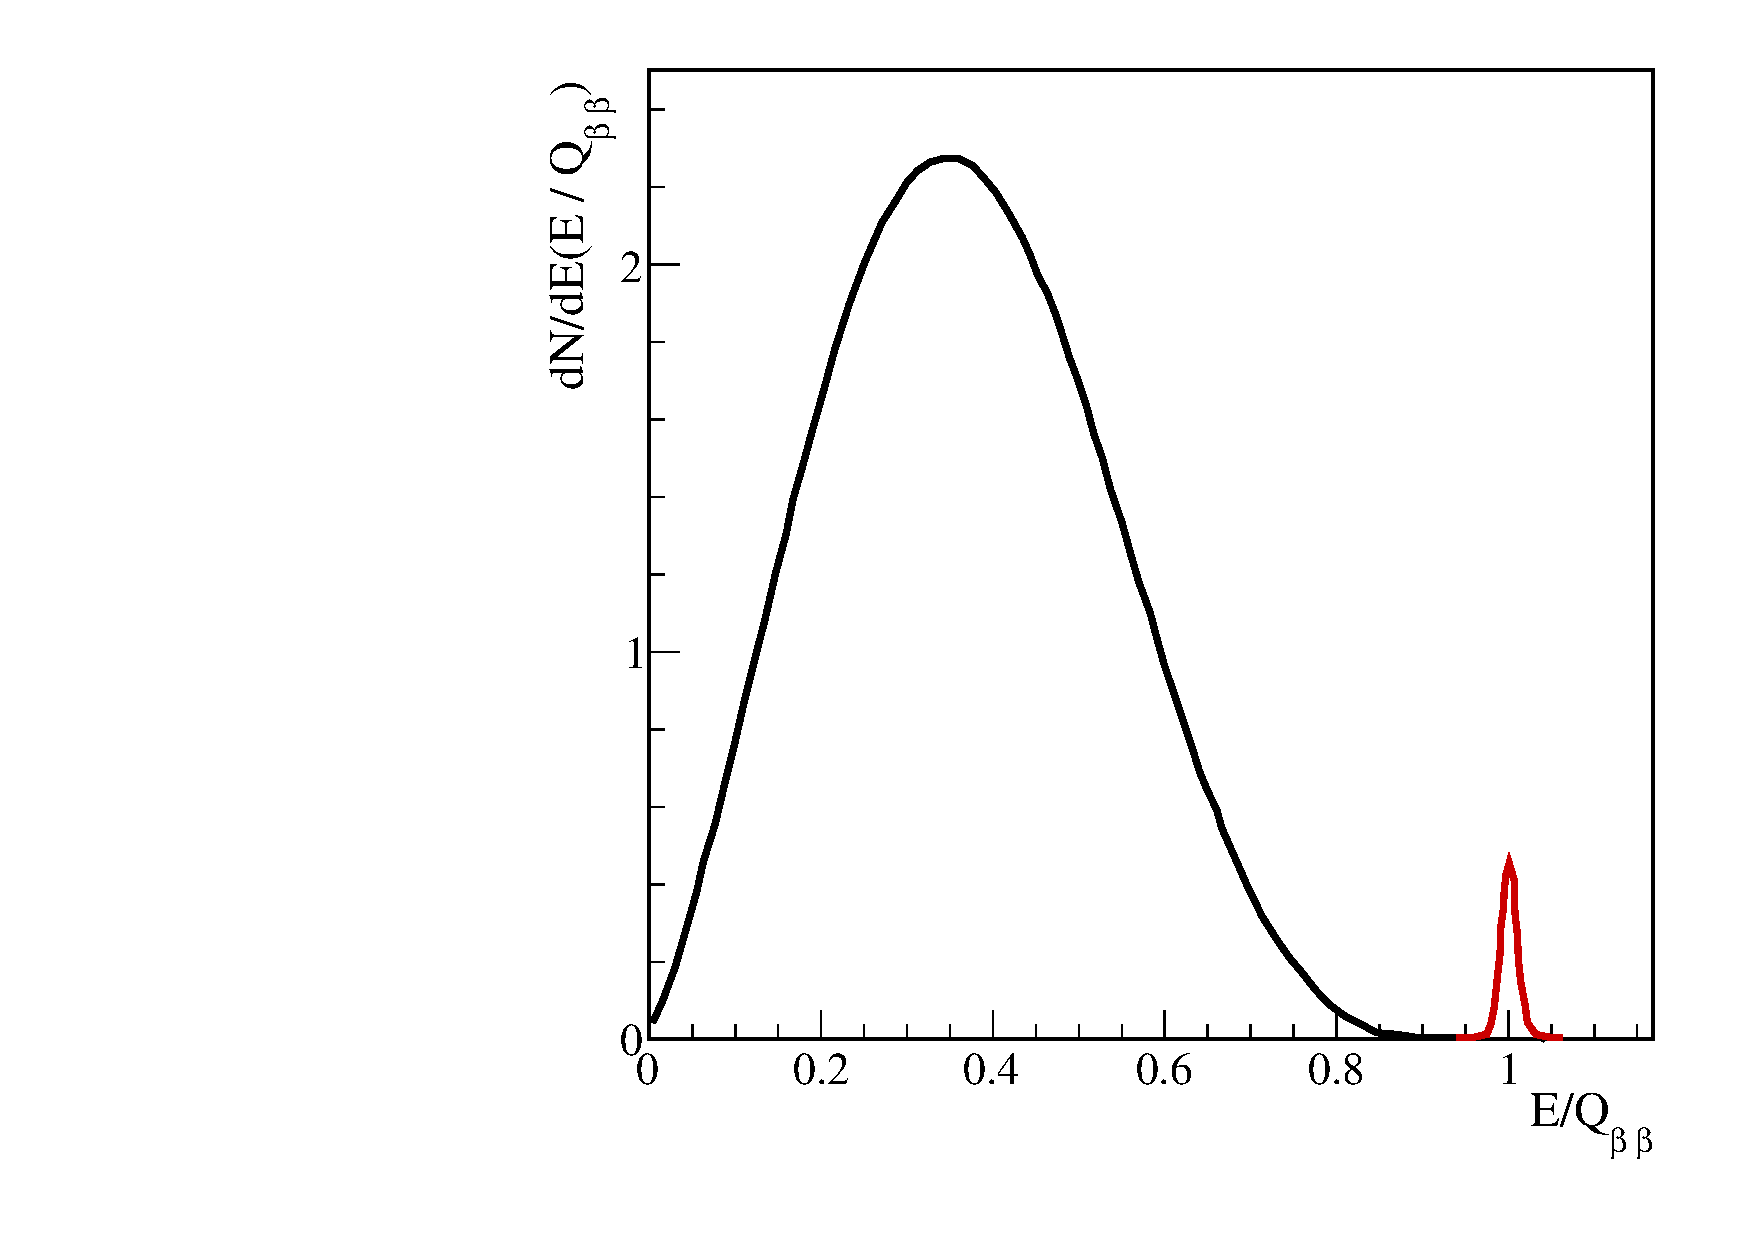
\includegraphics[width=0.25\columnwidth]{figs/CartoonBB.pdf}
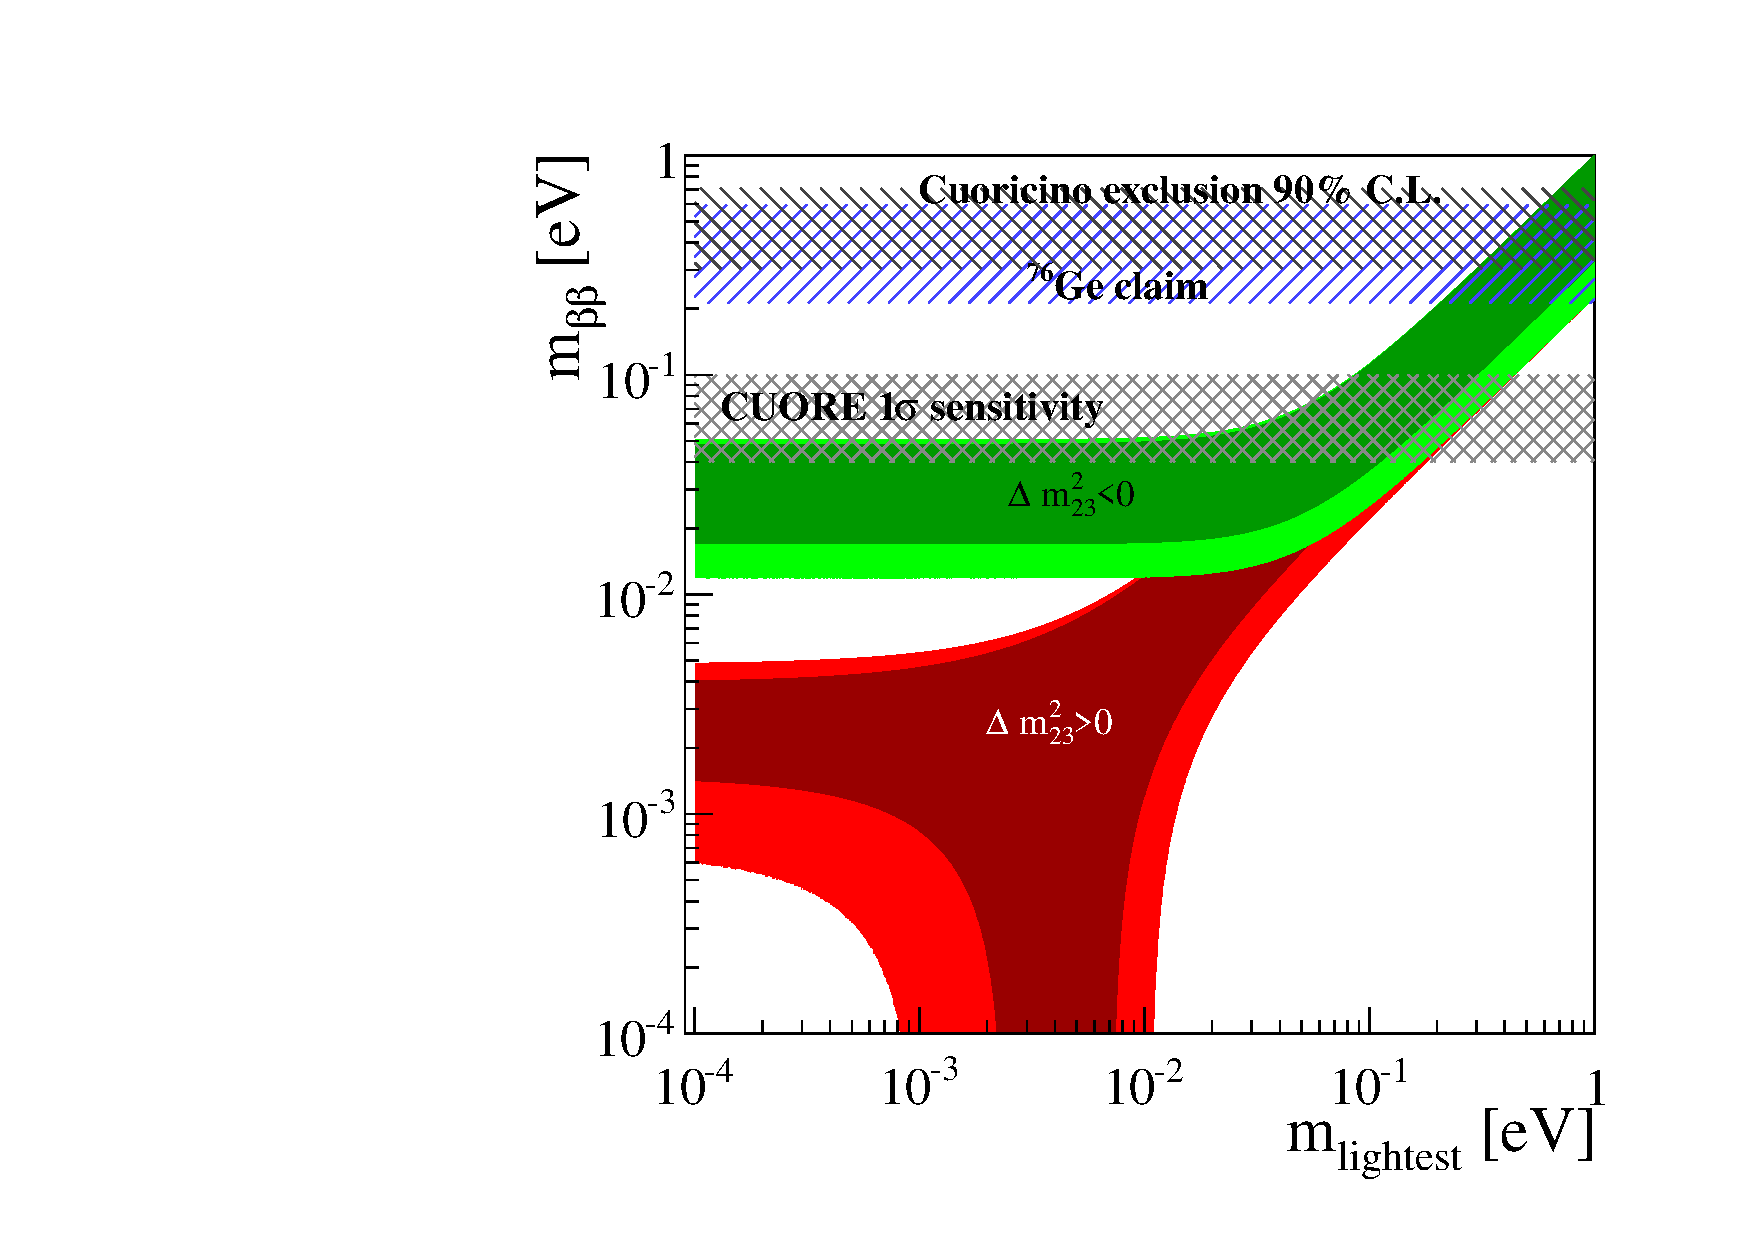
\includegraphics[trim=0.3cm 0.08cm 0.5cm 0.1cm, clip=true, width=0.26\columnwidth]{figs/M_bb_vs_m1_CL-2012.pdf} 
\end{center}
\caption{\footnotesize\label{fig0nuBB}  (Left) Feynman diagram for neutrinoless double-beta decay through light Majorana neutrino exchange. (Middle) Cartoon of the spectrum of electron energies from double-beta decay. The red section at the endpoint $Q_{\beta \beta}$ indicates those from neutrinoless double-beta decay\cite{RevBB}. (Right) The parameter space for \zeronu~as a function of the lightest neutrino mass  and the effective Majorana mass of the neutrinos, $m_{ee}$ \cite{Alessandria:2011rc}. }%The CUORE experiment will be the first to push into the inverted hierarchy. \cite{Alessandria:2011rc}.}
\end{figure}

The main mechanism for \zeronu~is the exchange of a light Majorana neutrino, as shown in Fig.~\ref{fig0nuBB} (Left).  This process is observable in isotopes where the single-beta decay to the Z+1 nucleus is kinematically forbidden so only the double-beta decay to the Z+2 nucleus is possible. The observed signal will be an excess of events at the endpoint of the \twonu~decay spectrum, see Fig.~\ref{fig0nuBB} (Middle). These experiments measure the half-life of  the \zeronu~decay:
\begin{equation}
\label{half0nu}
(T_{1/2}^{0\nu})^{-1} = G_{0\nu}(Q_{\beta\beta}, Z) | M_{0\nu}|^{2} \langle m_{\beta\beta} \rangle^{2}.
\end{equation}
$G_{0\nu}(Q_{\beta\beta}, Z)$ is the phase space available to the decay. $M_{0\nu}$ is the nuclear matrix element  for the decay. The last term is the effective Majorana mass of the neutrino,
\begin{equation}
m_{\beta\beta}= \sum_{i} U^{2}_{e i} m_{i}=\cos^{2}\theta_{13} ( m_{1}e^{2i\xi_2}\cos^{2}\theta_{12} + m_{2}e^{2i\xi_{1}}\sin^{2}\theta_{12})+m_{3}\sin^{2}\theta_{13}
\end{equation}
The sensitivity of \zeronu~experiments is plotted in terms of $m_{\beta\beta}$ versus the lightest neutrino mass eigenstate. Fig.~\ref{fig0nuBB} (right) is the expected sensitivity of the CUORE experiment. The sensitivity has a width due to the uncertainty in the nuclear matrix elements. The parameter space has an intrinsic width due to the interference of the two phases that contribute to \zeronu. There are two distinct regions corresponding to the inverted hierarchy for neutrino mass, the green region in  Fig.~\ref{fig0nuBB} (right)  and that corresponding to the normal hierarchy, the red region in  Fig.~\ref{fig0nuBB} (right). CUORE will be one of the first experiments to push into \zeronu~parameter space for the inverted hierarchy.

The sensitivity shown in Fig.~\ref{fig0nuBB} is the result of a detailed calculation\cite{Alessandria:2011rc}; however,  the sensitivity of a \zeronu~experiment can be approximated as\cite{sens0nu}
\begin{equation}
\label{sens0nu}
T_{1/2}^{0\nu}(n_\sigma) = \frac{4.16\times 10^{26} yr}{n_\sigma} \left ( \frac{\epsilon a}{W} \right ) \sqrt{ \frac{Mt}{b\Delta(E)}}.
\end{equation}
In this approximation, $n_\sigma$ is the number of standard deviations for the resulting half-life, $\epsilon$ is the detector efficiency, a is the isotopic abundance, and W is the molecular weight of the source material. It is the next terms that truly distinguish experiments: M is the total mass of the source, t is the duration of the experiment, b is the background rate in the region of interest in counts/(keV kg yr), and $\Delta(E)$ is the energy resolution. The energy resolution is key in distinguishing signal from backgrounds, especially background from the standard model process two-neutrino double-beta decay  (\twonu). 

It is the energy resolution that is the great strength of solid state detectors like CUORE and if a signal is detected will give us confidence that we have observed \zeronu. The PI is also interested in the question of how to scale \zeronu~detectors to access the parameter corresponding to the normal hierarchy. Although they suffer from poorer energy resolution liquid scintillator detectors scale well to large masses. In work supported by a different proposal, the PI  leads an R\&D effort to combine picosecond photodetector timing with novel liquid scintillators based on nanocrystals called quantum dots to extract a directional signal in this type of detector\cite{qdot,qdot2013,direction2013}. A directional signal has never been extracted from a scintillator detector and therefore the promising simulation results in Ref.~\cite{direction2013} are very exciting. These combined CUORE and liquid scintillator R\&D efforts form a coherent program to search for \zeronu~throughout the available parameter space.  The focus of this proposal is the support the PI's involvement in the CUORE experiment.

\subsection{CUORE Experiment}

\begin{figure}
\begin{center}
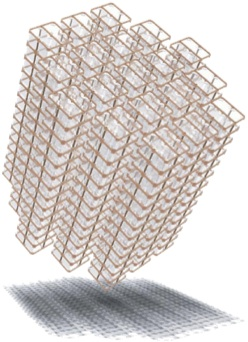
\includegraphics[width=0.225\columnwidth]{towers.jpg} 
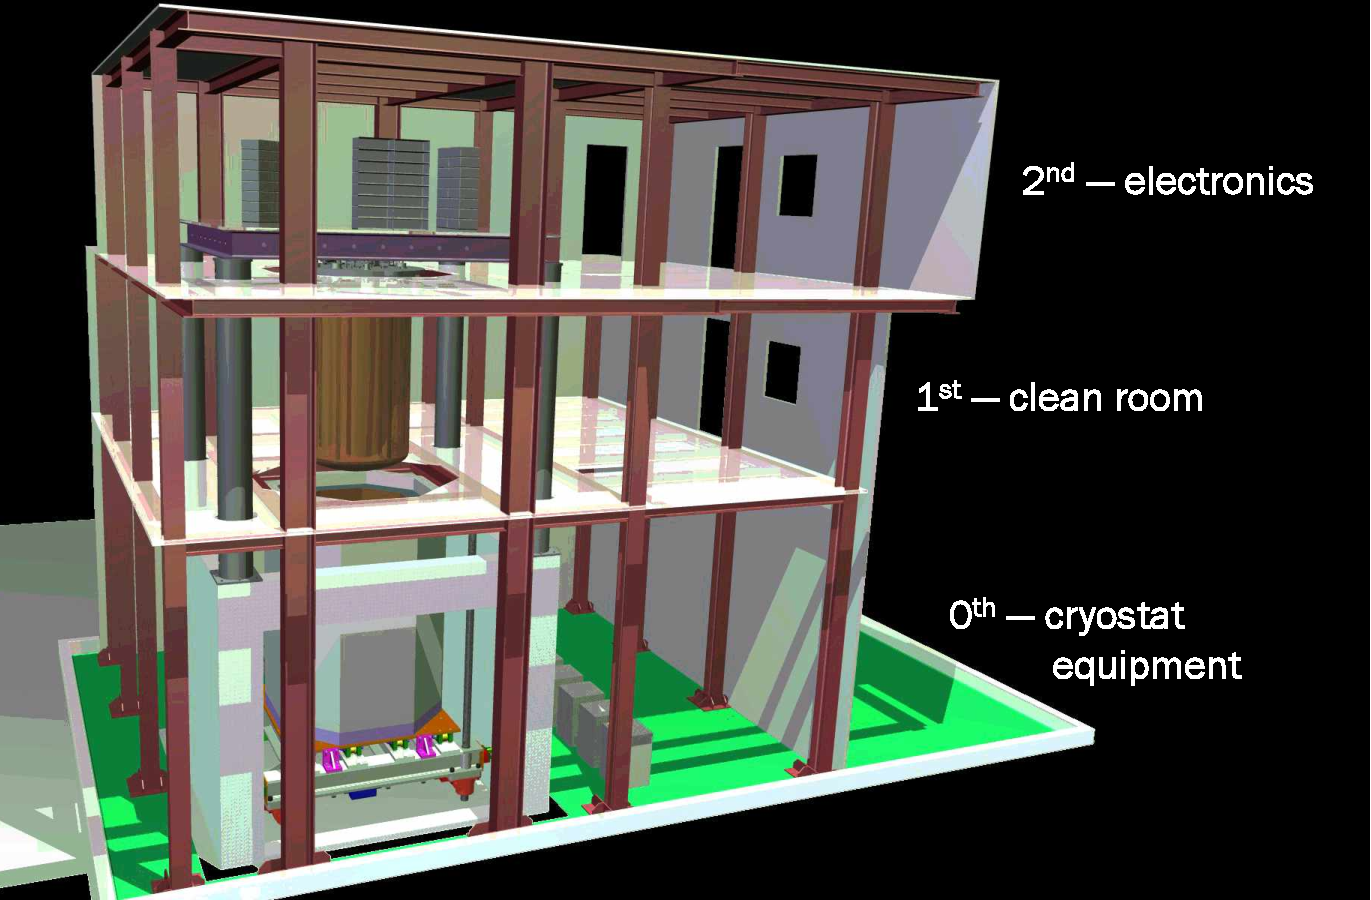
\includegraphics[width=0.505\columnwidth]{CUORE-hut-cross-section-labeled.pdf} 
\end{center}
\caption{\label{layoutCuore} The CUORE detector: the arrangement of the crystals into 19 towers (left) and the layout the CUORE detector in its clean hut (right).  }
\end{figure}

The CUORE experiment is searching for \zeronu~in $^{130}$Te with an endpoint of 2.527~MeV. Examining the terms in Eq.~\ref{sens0nu}, the advantages of this isotope and technology become obvious. The natural abundance is 33.8\% which means isotopic enrichment is not necessary. The only the gamma ray from the U/Th chains above the endpoint energy is the 2.6~MeV gamma ray from the decay of $^{208}$Tl.  The detector is constructed out of crystals of TeO$_{2}$  operated at 10~mK as bolometers. The CUORE crystals have achieved energy resolutions of 1.5~keV at the endpoint energy. This is on a par with all but the best germanium detectors. 

The performance of these crystals is the result of a 30-year program of experiments searching for \zeronu~with TeO$_{2}$ bolometers first proposed by Fiorini and Niinikoski  in 1984\cite{Fiorini198483}. It is the background levels which benefit most from this vast experience in crystal growth, mechanical support, readout, and handling, in addition to expertise in cryostat construction. The immediate predecessor of CUORE is the CUORICINO experiment, which ran from 2003-2008.  CUORICINO achieved a background level of 0.15 counts/(keV kg yr) in one tower of crystals representing 11.3~kg of isotope. They were able to set a limit of $T_{1/2}^{0\nu} > 2.8\times10^{24}$yrs at the 90\% C.L.

In order to improve upon this limit, the mass of the detector will be increased to 741~kg, representing  206 kg of isotope. The crystal dimensions are 5$\times$5$\times$5~cm$^{3}$ and they will be arranged into 19 towers as shown in Fig.~\ref{layoutCuore} (left). This factor of 20 increase in size is complemented by a factor of 20 reduction in the background levels through better choices of materials for the cryostat and mechanical supports, and better crystals handling. The first indications of success in background reduction are coming in now as the first data from CUORE-0 is analyzed by the collaboration. CUORE-0 is the first production tower of crystals for CUORE operated in the CUORICINO cryostat. A preliminary analysis presented at TAUP2013, the background level is 0.074$\pm$0.012 counts/(keV kg yr) , a factor of 2 reduction from the CUOROCINO background level of 0.153$\pm$ 0.006 counts/(keV kg yr).  With backgrounds on the order of 0.05 counts/(keV kg yr), CUORE-0 will be sensitive to $\langle m_{\beta\beta} \rangle$ between 0.17-0.39~eV. This is comparable to the current limits from EXO 0.14-0.38~eV\cite{EXO2012}, KamLAND-Zen combined with EXO 0.12-0.50~eV\cite{KZ0nu}, and GERDA 0.2-0.4~eV\cite{gerda2013}.  The full CUORE detector should then push down to 0.041-0.095~eV and begin to explore the inverted hierarchy.

As CUORE-0 runs, the rest of the towers are being constructed, and they will be installed by the end of 2014. The crystals are read out using Neutron Transmutation Doped (NTD) Ge thermistors. The assembly is labor-intensive, and one reason is that the NTDs are glued to each crystal individually. Therefore, all collaborators will be needed to help in this effort and in shift taking on CUORE-0. In parallel, the cryostat will be commissioned and integrated with the calibration system. The final configuration of the front-end electronics is being finalized now and everything is on schedule for data taking and first results from the full CUORE in 2015.

\subsection{Commissioning and Analysis Manpower}

The preliminary CUORE-0  analysis presented at TAUP2013 was a valuable exercise not only because it provided the first confirmation that the crystal handling procedures were achieving the desired background levels, but because it also tested the available manpower for the CUORE commissioning and analysis.  The analysis was performed by the equivalent of 2.5 postdocs and two graduate students: Jon Ouellet on data quality and Brian Zhu on MC background analysis. This was a combined U.S. and Italian analysis. Compared to similar experiments with multiple analysis teams and looking to the future with the the jump to almost 1000 channels, we are critically understaffed.  There has been a large U.S. investment in the construction of CUORE and we need to ensure that we have the manpower to extract all the excellent physics that can come from this multipurpose detector.

The MC is a self-contained task that exemplifies the current issues.  The full CUORE MC is an extension of the CUORICINO MC. The advantage is that much of the physics has been verified, and geometry has been implemented, however the output is a simple text file of energy deposition and crystal number. This is both an infrastructure issue since with the bigger detector and higher statistics the text file will become unwieldily.  This is also an issue for the sophistication of the analysis. Much more information can be extracted from the MC, but a more complex output format, usually ROOT-based,  is needed to capture this information. More manpower is needed to implement upgrades to the MC and do the MC data background verification. The postdoc supported by this grant will take on the leadership for this task.

The other metric by which CUORE manpower is insufficient is the number of graduate students. Graduate students are critical for completing the details of an analysis including studies of data quality and the evaluation of efficiencies. As is shown in Table~\ref{studentManPower}, there are currently only 1.5 U.S. graduate students  funded for CUORE-0 and 4 students for the full CUORE. The experiment is rich in thesis topics. Even with the addition of the graduate student funded by this proposal, there are topics not covered including the search to double-beta decay modes to excited states and the low threshold analysis which is sensitive to a direct dark matter signal. Our Italian collaborators have an even smaller number of students. Once again given the investment in CUORE,  and its physics potential in the next few years, now is the time to increase the number of graduate students and postdocs to ensure that the experiment reaches its full potential. As will be discussed in the following sections, the PI's group at UCLA is well positioned to contribute to the CUORE effort and brings the needed manpower at a critical time. The group has the support of the experiment, please see the attached letter from the U.S. spokesperson.

\begin{table}
\footnotesize
\begin{center}
\begin{tabular}{ l l l l l}
\hline
Student & Institution & Analysis & Graduation & Funding \\
\hline
Jon Ouellet & UC Berkeley & \zeronu~CUORE0 & 2015 & Yes \\
Brian Zhu  & UCLA & \zeronu~CUORE0 & 2015 &  1 year  \\
Nick Chott  & USC & Axion via Primakoff  conversion & 2018 & Yes \\
Nelson Camilo Posada-Aquirre  & USC & Axion via axio-electric effect  & 2018 & Yes \\
Alexey Drobizhev & UC Berkeley & \zeronu~CUORE & 2018 & Yes \\
Jeremy Cushman  & Yale &  \zeronu~CUORE & 2017 & Yes \\
Erin Hansen & UCLA & Majoron Decay CUORE & 2019 & {\bf This Proposal} \\
\hline
\end{tabular}
\caption{\label{studentManPower} Summary of U.S. students working on CUORE}
\end{center}
\end{table}


\section{Prior Results}

The PI's group at UCLA focuses on low energy neutrino physics and is currently concentrating on the search for \zeronu. This interest grows from the PI's experience on the Double Chooz and KamLAND experiments. The PI has a strong track record in producing physics results with 13 publications in the last two years.  The publications that are especially relevant are summarized in Refs~\cite{isodar,isodarscatt,pontecorvo,kamboron,qdot,qdot2013,direction2013,dcone,dctwo,dchydrogen,takahama}. The group is involved in three projects. The CUORE effort is the more mature effort. The other main effort is R\&D for next generation liquid scintillator detectors. Looking to the future, the PI is also working on the DAE$\delta$ALUS proposal especially the precursor experiment IsoDAR.

\subsection{Next Generation Liquid Scintillator for Double-Beta Decay}
If it becomes necessary to search for \zeronu~parameter space corresponding neutrino mass in the normal hierarchy then detectors with great than 10~tons of isotope will be needed. At these sizes, liquid scintillator detectors may become the superior technology due to the ease of scaling to large volumes\cite{biller}. Liquid scintillator detectors have poor energy resolution compared to solid state detecttors like bolometers. If a a directional signal could be reconstructed liquids scintillators would be come even more attractive, as the directional signal provides a method of background subtraction and opens the possibility to search for new physics in the angular correlation of the emerging electrons\cite{newphysics0nuBB}.  

The extraction of a directional signal requires improved photodetector timing. The directional signal is further improved by liquid scintillators with more narrow emission spectra.  In the last year, this effort has seen significant progress:
\begin{itemize}
  \item Building on the results in Ref.~\cite{qdot}, the chemistry of nanocrystals called quantum dots has been explored for novel liquid scintillators\cite{qdot2013}. New quantum dots have been identified and a collaboration with the Weiss lab in the department of chemistry has been formed. 
  \item A Monte Carlo was developed to understand what parameters affected the signal. Reconstruction algorithms from water Cherenkov detectors were then modified and applied to the Monte Carlo output. In Ref.~\cite{direction2013}, we show for the first time that it is possible to reconstruct the direction of $\sim$MeV electrons in a liquid scintillator detector.
  \item A prototype 1~m$^{3}$ detector has been designed. If funded it would be used to test the results obtained in Ref.~\cite{direction2013} and would be one of the first applications of the new picosecond photodetectors, the LAPPD\cite{LAPPDSum,LAPPDTDR}.
\end{itemize}
This work is to be supported by a different award, but is complementary to the work on the CUORE experiment.

\subsection{DAE$\delta$ALUS  Cyclotron Development}

The PI is also involved in the DAE$\delta$ALUS program which is developing cyclotrons for the production of neutrino beams\cite{Alonso:2010fs,daedaluswhite}. The full DAE$\delta$ALUS complex would produce a pion decay-at-rest (DAR) beam from three locations to search for the oscillation signal due to the CP violating phase $\delta$.  The injector cyclotron for the larger cyclotrons needed to produce the pion DAR can be used to produce an isotope DAR beam. When paired in close proximity to a kiloton-scale liquid scintillator detector a sterile neutrino search can be performed. This is the IsoDAR proposal\cite{isodar}. The PI has been particularly involved in the planning of IsoDAR, especially if situated at the KamLAND detector. 

The IsoDAR proposal has moved forward rapidly in the last year. The PI's involvement has been:
\begin{itemize}
 \item Coordinating between the two collaborations especially details of the infrastructure at the KamLAND. This includes identifying a location for the cyclotron and the accompanying beam dump.
 \item Coordinating the calculation of possible activation of materials especially the rock surrounding the cavity for the beam dump. This is a critical calculation due to the close proximity to the low-background KamLAND detector and the regulation for material activation in Japan.
 \item Analyzation of the backgrounds for a very promising neutrino scattering measurement that could be done in conjunction with the sterile neutrino search, see Ref.~\cite{isodarscatt}.
 \item Participation in and subsequent analysis of the ion source tests at BEST Cyclotrons with undergraduate Ruben Gutierrez.
\end{itemize}
This is a maturing effort. At this time the PI requests funds for one international trip to nurture the IsoDAR/KamLAND collaboration and the funds to support one undergraduate researcher. Since the experiment is in the proposal stage, there are many small analysis that make excellent self-contained projects for undergraduate researchers. There will also be additional measurements at BEST cyclotrons. Participating in the first round of testing was a great experience for Gutierrez and he gained unique experience with a real test beam.  It would be excellent for another undergraduate to gain similar experience.

\subsection{Double Chooz and KamLAND}
Before starting the group at UCLA, the PI gained much hardware and analysis experience through their work on the Double Chooz and KamLAND experiments.
The main hardware experience comes from the following projects:
\begin{itemize}
  \item Double Chooz Slow Monitoring System - The PI lead the commissioning and integration of the slow monitoring system into the Double Chooz data acquisition system. A wide range of hardware was included in this system from remotely operated power strips, to radon counters, and temperature and humidity sensors. A key part of the system was a custom instrumentation package consisting of magnetometers and temperature sensors that was installed with the PMTs inside the main detector. The data was readout using a variety of programs, but was collected in a central MySQL server administered by the PI. The data was also sent in real time to the custom JAVA based data viewer that the DAQ and other systems were using to control the experiment and send alarms to the shift takers. 
  \item Prototype Directional Neutron Detector - The PI lead an effort to refurbish a prototype directional neutron detector based on time projection chamber (TPC) for operation at the Double Chooz site. The details of this detector can be found in Ref.~ \cite{Lopez201222}. Fast neutron backgrounds are ubiquitous to low background experiments and is the most uncertain of the main backgrounds for Double Chooz's reactor antineutrino analysis of the oscillation parameter $\theta_{13}$\cite{dcone,dctwo,dchydrogen}. The data points at the Double Chooz near and far sites will be valuable for tuning Monte Carlo simulations. The full-scale version of this detector was recently completed by the PI's colleagues at MIT and it will start taking data shortly.  
  \item KamLAND Full Volume Calibration System - The largest detector systematic uncertainties on KamLAND's antineutrino analysis of the oscillation parameters $\theta_{12}$ and $\Delta m_{21}^{2}$ are the positions dependence of the position and energy reconstruction\cite{Eguchi:2002dm,Araki:2004mb,Abe:2008aa,Gando:2010aa}. The PI was the lead graduate student on the full volume calibration system that allowed the positioning of radioactive sources everywhere with the fiducial volume\cite{fourpi}. The PI was responsible for the instrumentation packages that were deployed as part of the system and the cleaning procedure that ensured that the deployment of the system did not significantly increase the radioactive backgrounds from the U/Th daughters in the detector. 
\end{itemize}

The PI's hardware experience especially the slow monitoring work is directly applicable to the proposed work in this award. Similarly, the PI's analysis experience is highly relevant to the proposed analysis focus:
\begin{itemize}
  \item Double Chooz U.S. Analysis Coordinator - The U.S.-based analysis cluster, Cluster United, developed an analysis for $\theta_{13}$  that utilized the antineutrino rate and spectral shape. The analysis propagates the uncertainties on the energy scale using detailed comparisons of the calibration data  and the Monte Carlo. It is this analysis that is published in Refs.~\cite{dcone,dctwo,dchydrogen}. The PI also worked closely with the reactor simulation group and lead the effort to benchmark the reactor simulation codes against actual data from the Takahama reactors\cite{takahama}.
  \item Double Chooz Data and Monte Carlo Production Leader - The PI developed tools with MIT graduate student Kazuhiro Terao based on a MySQL database to process and track data as it arrived at the experiment's analysis cluster. These tools were also used to organize the Monte Carlo production. In addition, he PI wrote the event generator for the decay of beta-delay neutron emitter $^{9}$Li. This is a complicated decay with a fair amount of uncertainty in the input branching ratios and widths of excited states that must be evaluated and correctly propagated to the $\theta_{13}$ analysis.
  \item KamLAND Spallation Analysis Leader - Closely related to fast neutron background, the production of unstable isotopes through muon spallation is ubiquitous to low background experiments. The was one of the leaders of the KamLAND spallation analysis and was particularly responsible for the simulation results using FLUKA\cite{kamspall}. These results expanded the spallation products used to benchmark simulations beyond neutrons for the first time. 
\item KamLAND $^{8}$B Solar Neutrino Analysis Leader - The main analysis on KamLAND is the reactor antineutrino analysis, but KamLAND is also sensitive to solar neutrinos through neutrino-electron scattering. This analysis is more difficult because it does not have the coincidence signal that reduces backgrounds so effectively in the antineutrino analysis.  By doing a detailed accounting of the backgrounds that contribute to single events in the detector, especially the spallation backgrounds, a measurement of the $^{8}$B solar neutrino flux was extracted\cite{kamboron}. The results is in agreement with the very precise Super-Kamiokande measurements\cite{skboron}, and those from SNO\cite{snoboron} and Borexino\cite{borexinoboron}. 
\end{itemize}

\section{Proposed Research Plan}

\subsection{Hardware Focus: Slow Monitoring}
The main components of the CUORE detector are the crystals, their electronics, the cryostat to cool the crystals to their 10~mK operating temperature, and the calibration system, which is a wire based system to move sources in and around the crystals. This is all being assembled in a three-story-hut,  Fig.~\ref{layoutCuore} (right), underground at the Laboratori Nazionali del Gran Sasso. Although Gran Sasso is one of the most convenient underground laboratories in which to work, access is not always guaranteed. For this reason, a robust remote monitoring system for all detector components and the surrounding environment is needed. The collaboration has identified this as a critical task within the project for the new UCLA group to lead.

The task has two parts: unifying the slow monitoring and the interface to the data from the various devices that make up the detector, and providing hardware to monitor the environment including vibrations in the three-story CUORE hut. For measuring the environment, a hardware package needs to be constructed which can measure temperature, humidity, and radon levels.  One package is needed on each of the three floors of the hut, A netbook per floor is envisioned for reading out the systems plus a rack-mounted computer devoted to slow monitoring to run the main database and serve the data. This is very similar to the package and system put together for Double Chooz. 

The proposed package uses inexpensive radon counters purchased from AWARE Electronics\cite{aware} where the output pulses are then counted with the USB-CTR-15\cite{usbctr}.  The latter device has many spare channels for other devices from other systems that may need to be integrated into the slow monitor system. Unfortunately, the temperature and humidity sensors used on Double Chooz and KamLAND have been discontinued. There are several companies making TCP/IP-readable packages, ranging from \$60 to \$200 depending on the sophistication of the readout. Depending on the air-conditioning system, more thermometers may be needed, so the upper estimate is used in the budget summarized in Table~\ref{slowRequest}. 

The monitoring of vibrations may be particularly interesting since vibrations of the crystals represent one of the larger factors contributing to the energy resolution\cite{vignati}. Vibrations are characterized by their frequency, direction, and magnitude. Accelerometers to measure vibrations come in a wide range from very inexpensive surface mount components to complex systems which output the frequency spectrum in real time. The more complex system is needed to characterize the vibrations present in the CUORE hut. The characterization of the vibrations and their correlation to CUORE data makes an excellent project for a graduate student to lead. We propose to purchase a 3-axis accelerometer from  Br\"{u}el \& Kjaer\cite{bk}  with its accompanying DAQ for this project. Once this study is complete a simpler system could be designed or if necessary additional 3-axis accelerometers may be added to the  Br\"{u}el \& Kjaer. We note that CUORE has been designed to isolate the crystals from external vibrations, but at what level they will contribute is an open question.

\begin{table}[position specifier]
\begin{center}
\begin{tabular}{ l c l}
\hline
Equipment & Number & Cost \\
\hline
Br\"{u}el \& Kjaer Accelerometer and DAQ & 1 & \$13500.00 \\
Netbook & 3 & \$1000.00\\
Temp. \& Humidity & 3 & \$500.00 \\
USB-CTR-15 & 3 & \$1000.00\\
Radon Counter & 3 & \$1200.00\\
Additional Sensors & - & \$800.00 \\
\hline
Total & & \$18000.00 \\
\hline
\end{tabular}
\caption{\label{slowRequest}The budget for environmental monitoring for CUORE. The estimate for the slow monitoring server is from a recent purchase of a dual six-core 2.66Ghz 48GB system. Spares are requested to facilitate debugging at UCLA and allow for quick shipment to site. These costs are unloaded.}
\end{center}
\end{table}

The second half of this task is the centralization of the slow monitoring data. The most critical device to monitor is the cryostat, which is read out via LabVIEW. The calibration system and several other miscellaneous devices have internal TCP/IP servers for communication, while several older devices still communicate via RS232. The software package that manages these devices must have the infrastructure to build interfaces to these devices, provide infrastructure to process data and set alarms, and finally provide a user interface such as a graphical user interface (GUI) or a webpage for shift taking. This sort of software package is called a Supervisory Control And Data Acquisition package (SCADA). The PI has taken part in writing a custom SCADA package for Double Chooz. There are also several open-source packages that have been developed for operating physics experiments. Based on the PI's experience, an open source package is the more time-effective option.

The software packages that were considered were  EPICS\cite{epics}, MIDAS\cite{midas}, TANGO\cite{tango}, TINE\cite{tine}, and ORCA\cite{orca}.  Most of these packages come from the accelerator community, except for ORCA, which has been developed primarily for the Majorana program. ORCA is a Mac-based system, and at this point it may not be possible to port it to CUORE.  Our Italian collaborators have close ties to the TANGO developers. TANGO also has a well documented LabView interface. For this reasons, it was decided to base the new CUORE system on TANGO. An example TANGO  system has been setup at UCLA and computer science graduate student Pranay Doshi has written a python based user interface for computers and smart phones. We are now working to setup a TANGO network onsite and are evaluating the python interface and its future integration with other systems for shift taking especially the main DAQ.

\subsection{Analysis Focus: Monte Carlo and Exotic Double Beta-Decay Searches}
The great enthusiasm for double-beta decay searches comes from the fact that the observation of \zeronu~would prove that the neutrino is a Majorana particle. This has consequences for cosmology and models of leptogenesis, which use the heavy neutrino partners of light neutrinos to produce the matter-antimatter asymmetry in the universe. 

The main CUORE analysis is the search for \zeronu~moderated by a light Majorana neutrino.  However, other models exist for the double-beta decay of Majorana neutrinos. One group involves the ejection of a massless boson called a Majoron $\chi^{0}$. The observational signature of these models (\maj) is a change in the detected summed energy of the two electrons, as shown in Fig.~\ref{majoran}.  In the models where the decay is moderated by a light Majorana neutrino, the sum of the electron energy is the endpoint energy broadened by the detector resolution. The \maj~models show a broadened spectrum corresponding to the sharing of the energy among the electrons and the $\chi^{0}$. 

\begin{figure}
\begin{center}
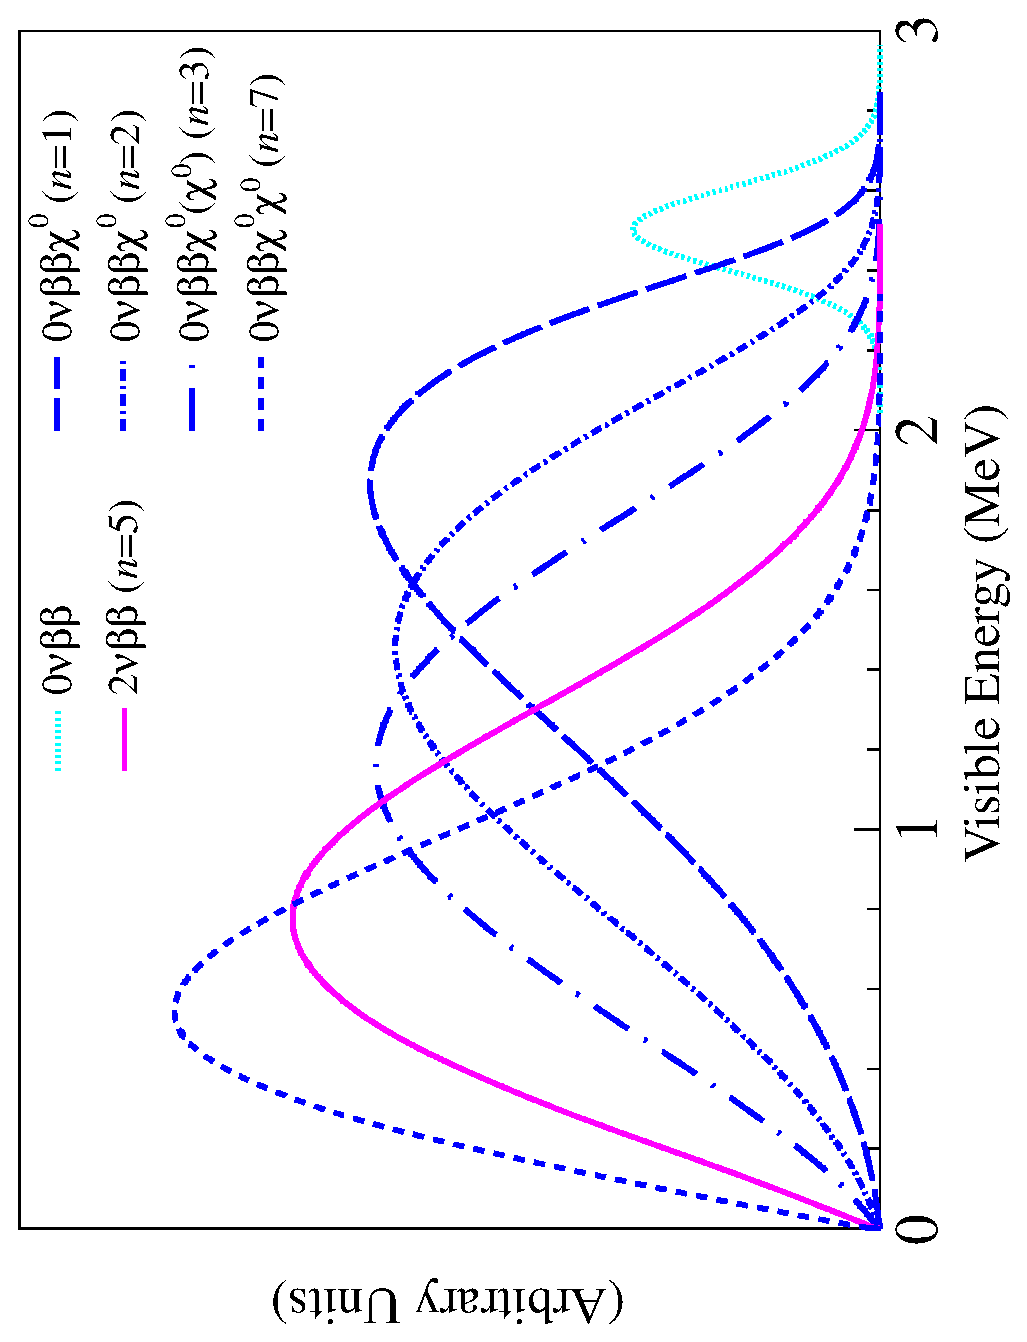
\includegraphics[angle=270, width=0.58\columnwidth]{fig1} 
\end{center}
\caption{\label{majoran}The effect of Majoron emission on the \zeronu~spectrum from Ref.~\cite{KZMaj}. The endpoint for \isoxe~is shown. The search in CUORE would be the same except centered at the \isomain~endpoint of 2.527~MeV. }
\end{figure}

The best limits on these models currently come from the KamLAND-Zen experiment, which puts limits on the half-lives in \isoxe~of $T_{1/2}^{0\nu\chi^0}>2.6\times10^{24}$~yrs at the 90\% C.L.\cite{KZMaj}. The best limits on this process in \isomain~are $T_{1/2}^{0\nu\chi^0}>1.6\times10^{22}$~yrs at the 90\% C.L. from the NEMO-3 experiment\cite{nemo3Te}. NEMO-3 is a tracking detector which allows for large reductions in backgrounds. Unfortunately, the measurement was still limited by backgrounds and had a signal to noise (S/N) of 0.5. CUORICINO did not search for these processes.

The measurement of the standard model process of two-neutrino double-beta (\twonu) is closely related to the $\chi^{0}$ search and is a background to the search. The \twonu~analysis was the thesis topic of the CUORICINO student Laura Kogler\cite{laura}. The background levels in CUORICINO were too high to extract the \twonu~rate by directly simulating and fitting the background shapes. In order to extract \twonu~half-life, a background subtraction was done using crystals depleted in~\isomain. This type of subtraction will not be possible in CUORE since there are no plans to run with crystals of different enrichments. The reduced background contamination is expected to bring the S/N up to 1.0. At this background level, a fit should be possible by directly simulating the background shapes. This would allow an improved measurement of the \twonu~rate, and a search for double-beta decay with $\chi^{0}$ ejection. In addition, the \twonu~measurement is interesting in itself as it can be used to understand the quality of the different nuclear matrix calculations. 

The search for \maj~requires a detailed model of the backgrounds and detector response in a larger portion of the energy spectrum than is needed for \zeronu. For this reason, it is critical to have proper infrastructure in place for running, analyzing and tuning the MC. As was mentioned earlier, CUORE has a Monte Carlo in place but upgrades to the infrastructure and manpower for analyzation and tuning are needed. It is logical that the group leading the \maj~analysis also take on leadership on the Monte Carlo. Furthermore, the MC improvement and other analysis tools developed for the \maj~analysis are directly applicable to the main \zeronu~analysis, so the group will also maintain a strong presscence on the main analysis.

\subsection{Group Plan}
This proposal's purpose is to support the participation of the PI, a postdoc, one undergraduate, and one graduate student on CUORE. A small amount of funds, one undergraduate researcher and one international trip,  to support work on future experiments including the DAE$\delta$ALUS/IsoDAR proposal. The general plan for the group is the slow monitoring work in the first year of the award, commissioning in the second year, and data analysis in the third year of the award. 

A strong group has already been assembled. The PI wanted to recruit a first year student and actually recruited two excellent students, Agnieska Wergieluk and Erin Hansen. It is a testament to the exciting physics that will be coming from CUORE in the near future that we were able to recruits these two students and are continuing to get inquires from others. Both  students spent summer 2013 at Gran Sasso. Wergieluk took CUORE-0 shift and worked to improve the shift documentation while beginning to learn the analysis tools. Hansen lead the crystal gluing for much of her time onsite, completing the gluing of thermistors to crystals for 1.5 CUORE towers, see Fig.~\ref{broad}. She also started to learn the analysis tools and put together tools for tracking the thermistors production information.Wergieluk is still deciding between theory and experiment. Hansen has decided to do her thesis on CUORE and would be supported by this award.

The entering class of graduate students at UCLA in 2012 was small, and therefore it is unlikely that the PI will find a graduate student before the start of the grant. Instead the PI would prefer to recruit a graduate student from the incoming group in 2013. The PI is particularly interested in recruiting one of three undergraduate researchers with CUORE experience who will graduate from Cal Poly San Luis Obispo this year. In year one and two of the grant, this student would be taking class; therefore, they would spend the summers onsite working on tower construction, taking CUORE-0 shift, and generally becoming an expert on the detector and CUORE-0 data analysis. During the academic year at UCLA, they would write the \maj~MC generator, and learn how to run the CUORE MC at UCLA's computing facility. In year three of the award, they should be ready to assist the postdoc with the search for \maj~ in the full CUORE data.

The postdoc is the critical member of the group. The integration of the slow monitoring needs a person to spend at least 50\% of their time onsite during the first year of the award to facilitate this process and to understand the needs of the detector as it is constructed. As one of the goals is to build an analysis group at UCLA, the postdoc will not be stationed onsite. Because of the low-level nature of the hardware work, a postdoc with experience in \zeronu~physics is preferred, so that they may  jump into the analysis quickly.  In addition to a general search, two candidates who could start in January have been identified, and are being recruited. This advertisement should be posted shortly. 

In the first year of the award, Hickerson will need to focus on the slow monitoring, but some time should be used to develop code to do the basic sensitivity study for the \maj~search. The second year of the award represents the apex of the CUORE commissioning, and Hickerson should be in the heart of this effort as the leader of the slow monitoring and a member of the UCLA electronics group. In this time, the results of the basic sensitivity study should be used to guide the background simulation efforts. The third year of the grant should have the first data from the full CUORE detector, and the analysis ready to run. Hickerson should be ready with the simulated backgrounds from a and should be in a good position to be a leader in the main analysis as well as the search for \maj. Most critically, this should also provide the postdoc the results that are needed for applying for a job in that year or the following one.

\section{Broader Impacts}

\begin{figure}
\begin{center}
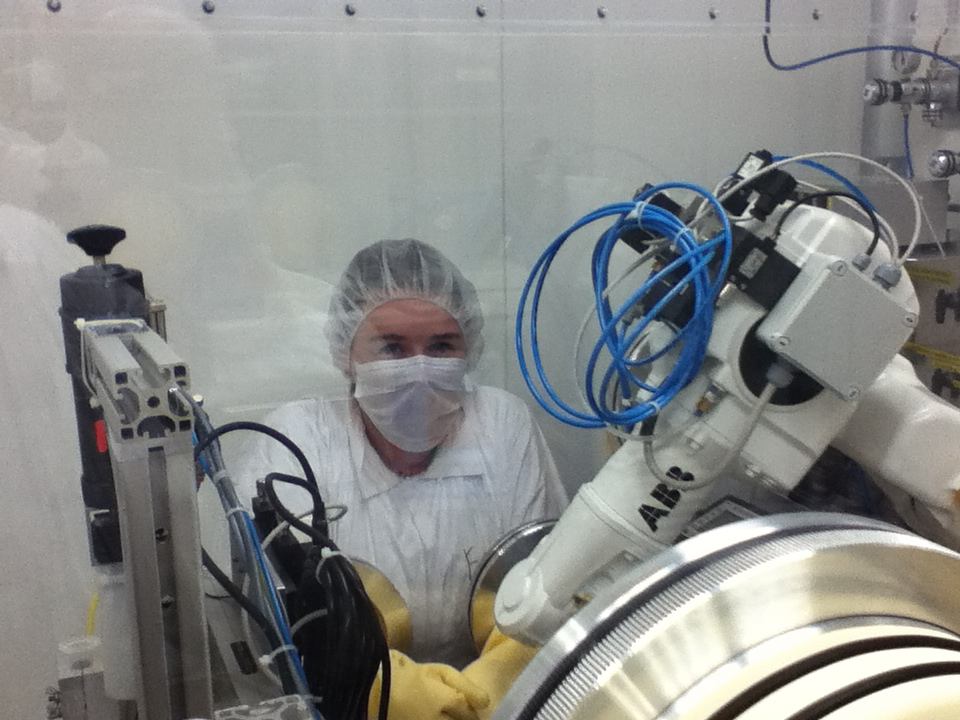
\includegraphics[width=0.35\columnwidth]{figs/Erin1.jpg} 
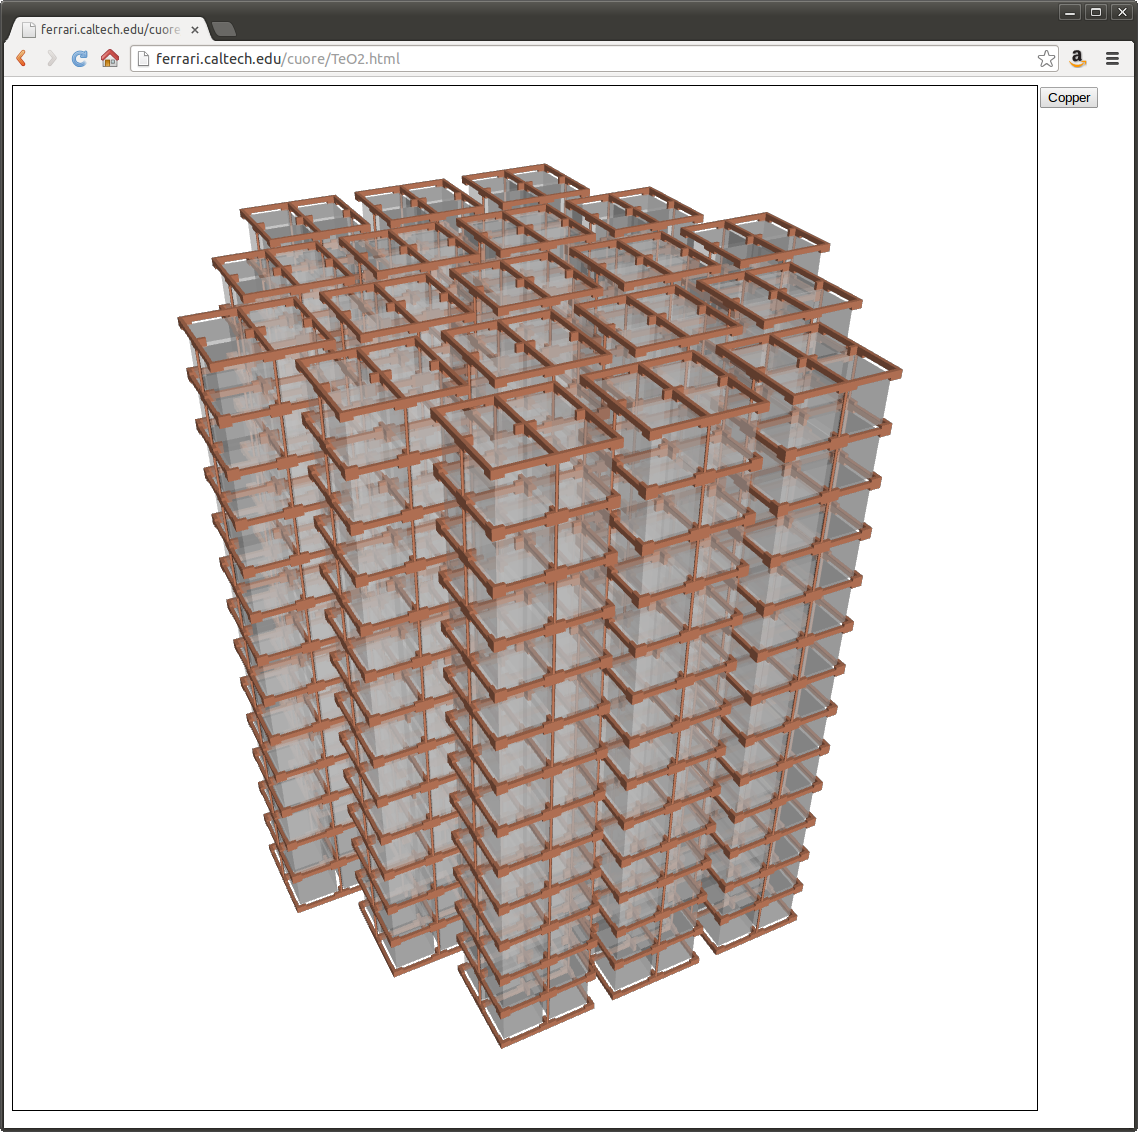
\includegraphics[width=0.3\columnwidth]{figs/viewerPlain.png} 
\end{center}
\caption{\label{broad} (Left) Graduate student Erin Hansen gluing thermistors as the gluing leader during the summer of 2013. (Right) Web-based visualization of the CUORE Monte Carlo. A series of button will allow the highlighting of different detector components and in the future will allow the creation of an event viewer for public outreach. }
\end{figure}

The broader impacts of this proposal are three-fold: training of students in nuclear physics, broadening the diversity of participation in physics, and public outreach through a web-based event viewer. The CUORE experiment provides training in nuclear physics for graduate and undergraduate students. The Nuclear Science Advisory Committee (NSAC) report on education in nuclear science from 2004 recommended a 20\% increase in the number of students trained in nuclear physics over the next 10 years to meet the needs of the U.S. workforce\cite{nuced}. The connection between the double-beta decay measurement and astronomy and cosmology captures the imagination of students and draws them into nuclear science, where they can learn why this is such an exciting field of study.The graduate student who will be supported by this grant is shown in Figure~\ref{broad}.

Secondly, the PI has a long track record of working to increase the participation of women
and minorities in physics. The PI's mentoring work with the MIT Summer Research Program was recognized with MIT"s Infinite Kilometer Award. The PI continues this work with enthusiasm at UCLA. The requested funds for two undergraduate students will give more undergraduates the opportunity to experience both the direct and indirect benefits of research. These students will takeover from current undergraduates Elizabeth Friedman on CUORE and Ruben Gutierrez on the IsoDAR proposal. The PI has advises fledgling graduate and undergraduate women in physics groups. Friedman is the founder of the undergraduate women's group and we are working together to arrange monthly lunches and for a group of UCLA undergraduates to attend the undergraduate women in physics hosted at UC Berkeley this winter.

%and mentored Athena Ierokomos as part of UCLA's REU program.
The third impact of this proposal will be the creation of a website explaining the CUORE experiment and its results for the public. The center piece of this website will be an interactive event viewer based upon the visualization of the CUORE Monte Carlo. A screenshot of the web-based viewer with one button to highlight the copper support is shown in Figure~\ref{broad}. The PI has worked on similar projects most recently a online course on neutrino oscillations as part of the Annenberg Foundation's \textit{Physics for the 21$^{st}$ Century}. The experiment currently does not have a description for the general public. The postdoc Hickerson is interested in integrating this project into his Monte Carlo work, and the composition of the experiment descriptiont is an excellent project for a beginning undergraduate.

The success of the broader impacts of this grant will be demonstrated in several ways.   First, by the end of the three-year grant, the goal is to ensure the new women in physics groups at UCLA have active ongoing programs.  Second, success will be defined by maintaining a diverse group and continuing to recruit minority students to the group. Currently, UCLA has a 10\% minority population within the physics major in which to advertise. However, one of UCLA's great strengths is its large hispanic community, 17\% of the undergraduate population. This represents a great recruiting opportunity for increased participation in the major. The success  of these students will be defined by the publication of papers and presentations at  conferences like APS April Meeting. We are excited to note that  Gutierrez obtained one of the Conference Experience for Undergraduate slots at DNP2013 and will be presenting his IsoDAR work there. Finally by the end of the award, a website for the public will be complete, centered around the interactive event display.

\section{Conclusion}
The neutrino is not quite as mysterious as it was a decade ago, but the physics questions are arguably more important. The first detection of neutrinoless double-beta decay will have great implications for mass generation in particle physics, but the ripples from such a discovery will be felt in the far corners of astrophysics and cosmology. The CUORE  detector is poised to probe deeper into the double-beta decay parameter space than any experiment that will turn on in the next few years, and its technology of TeO$_2$ bolometers is applicable to other measurements.

This technology is new to the PI, but their experience in other low background physics has prepared them well for this analysis. Specifically in the last two years, the PI has been one of the coordinators of the Double Chooz  analysis which has produced five analysis papers related to reactor antineutrinos and the measurement of $\theta_{13}$\cite{dcone, dctwo, takahama,Abe:2012gw,Abe:2012ar}. This work continues with several papers in progress including a search for \zeronu~in $^{160}$Gd. In this same period, the PI has also published several papers related to R\&D efforts and proposals for new experiments\cite{Alonso:2010fs,isodar,qdot,Lopez201222}.

This award mainly supports students and a postdoc on CUORE. The group's proposed hardware task of the slow monitoring builds on the PI's slow monitoring experience on Double Chooz and integrates the group with the greater CUORE effort. Similarly, the proposed analysis focus on searches for exotic double-beta decay modes builds on the PI's experience simulating backgrounds, gives the group a well defined task, but does not segregate the group from the main CUORE analysis. 

It is an exciting period for CUORE as the pieces are coming together, and data from the completed detector is on the horizon. This is a great time for a new group to join the experiment, especially one that has support at their home institution and in the greater collaboration. The PI is knowledgable in the field and is well positioned to lead a group towards interesting new physics. 
